\documentclass[aspectratio=169]{beamer}

\usetheme{metropolis}
\usepackage{appendixnumberbeamer}

\usepackage{booktabs}
\usepackage[scale=2]{ccicons}

\usepackage{pgfplots}

\usepackage{xspace}
\newcommand{\themename}{\textbf{\textsc{metropolis}}\xspace}

\usepackage[utf8]{inputenc}
\usepackage[T1]{fontenc}

\usepackage{listings}
\usepackage{xcolor, colortbl}
\usepackage{multicol}
\usepackage{chronology}

\usepackage[]{algorithm2e}

\definecolor{done}{rgb}{0.36, 0.72, 0.36}
\definecolor{doing}{rgb}{1.0, 0.8, 0.0}
\definecolor{scheduled}{rgb}{0.25, 0.54, 0.79}


\newcommand{\done}{\cellcolor{done}}
\newcommand{\scheduled}{\cellcolor{scheduled}}
\newcommand{\doing}{\cellcolor{doing}}

\bibliographystyle{unsrt}

\lstdefinestyle{sharpc}{language=[Sharp]C, frame=lr, rulecolor=\color{blue!80!black}}


\title{Eliminando Gargalos de Processamento \newline Utilizando Rust}
\date{}
\author{Johnathan Fercher}
%\institute{Braspag}
\titlegraphic{\hfill
\includegraphics[height=1.1cm]{imgs/logo.png}}

\begin{document}
\maketitle

\begin{frame}{Sumário}
  \setbeamertemplate{section in toc}[sections numbered]
  \tableofcontents[hideallsubsections]
\end{frame}

\section{Introdução}
\begin{frame}{Gargalos}	
	\begin{center}
		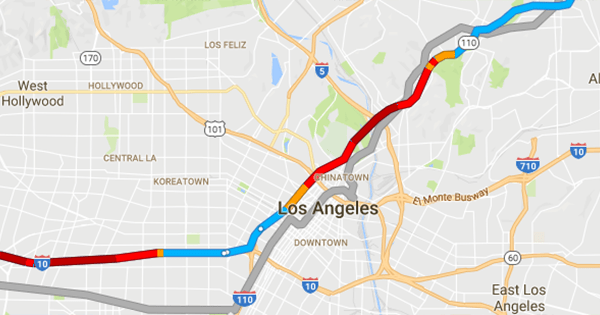
\includegraphics[width=7cm]{imgs/bottleneck}
	\end{center}
	\begin{itemize}
		\item Um gargalo é a parte menos eficiente de um sistema:
		\begin{itemize}
			\item 90\% de um trajeto é feito a 110 km/h e 10\% é feito a 20 km/h;
			\item Um caixa 24 horas dentro de uma loja que fecha;
		\end{itemize}
	\end{itemize}		
\end{frame}

\begin{frame}{Gargalos}	
	\begin{itemize}
		\item IO-Bound;
		\item CPU-Bound;
	\end{itemize}	
\end{frame}

\begin{frame}[noframenumbering]{Gargalos}	
	\begin{itemize}
		\item CPU-Bound:
		\begin{itemize}
			\item Utiliza todo o processamento, porém, ainda demora;
		\end{itemize}
	\end{itemize}	
\end{frame}

\begin{frame}[noframenumbering]{Gargalos}		
	\begin{itemize}
		\item CPU-Bound:
		\begin{itemize}
			\item $\rightarrow$ Algorithms, Parallel Programming, Programming Languages;
		\end{itemize}
	\end{itemize}	
\end{frame}

\begin{frame}[noframenumbering]{Gargalos}		
	\begin{itemize}
		\item CPU-Bound:
		\begin{itemize}
			\item $\rightarrow$ Algorithms, \textcolor{blue}{Parallel Programming}, \textcolor{blue}{Programming Languages};
		\end{itemize}
	\end{itemize}	
\end{frame}

\begin{frame}{Introdução}
	\begin{multicols}{2}		
		\begin{center}
			
\includegraphics[width=5cm]{imgs/rust3d.png}
		\end{center}
		\footnotesize
		\begin{itemize}
			\item Programming Language;
			\item Memory and thread-safe;
			\item Rust $\rightarrow$ LLVM $\rightarrow$ EXE;
			\item C-Bindings;
			\item Object-Oriented and Functional;
			\item Unit-tests and Package Manager;
			\item Interfaces and Generics;
			\item Without Garbage Collector;
		\end{itemize}	
	\end{multicols}
\end{frame}

\begin{frame}{Motivação}
	\begin{quote}
		\hspace{0.5cm}"O clock dos processadores dobra a cada 18 meses."
		
		\hspace{8.2cm}Lei de Moore, 1965.
	\end{quote}
\end{frame}

\begin{frame}[noframenumbering]{Motivação (Acha que isso ainda funciona?)}
	\begin{center}
		
\includegraphics[width=4.0cm]{imgs/choque_de_cultura_05.jpg}	
	\end{center}
\end{frame}

\begin{frame}{Motivação}
	\begin{center}
		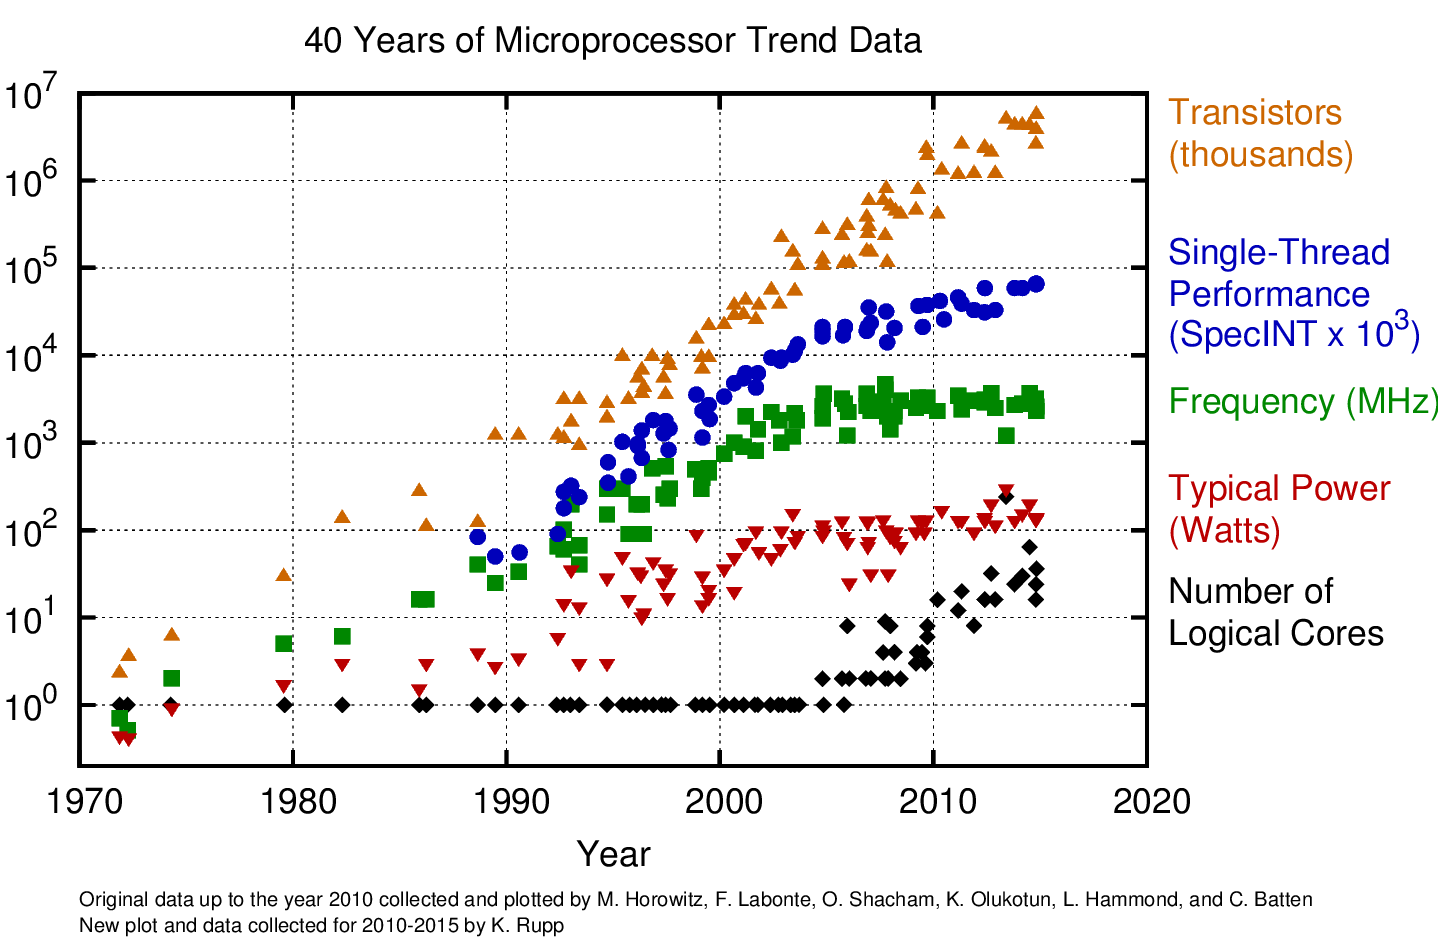
\includegraphics[width=12.5cm]{imgs/cores-history.png}
	\end{center}
\end{frame}

\begin{frame}{Motivação}
	\begin{quote}
		"The way the processor industry is going, is to add more and more cores, but nobody knows how to program those things. I mean, two, yeah; four, not really; eight, forget it."
		
		\hspace{8.2cm}Steve Jobs, Apple.
	\end{quote}
\end{frame}

\begin{frame}{Motivação}
	\begin{center}
		
\includegraphics[width=13.5cm]{imgs/bug.png}
	\end{center}
\end{frame}

\begin{frame}{História}
	\begin{chronology}[5]{2000}{2015}{80ex}[\textwidth]
		\event{2000}{LLVM}
		\event{2006}{Rust in OCalm}
		\event{2009}{Mozilla}
		\event{2010}{Rust-c in Rust}
		\event{2011}{Rust-c using LLVM}
		\event{2012}{Alpha}
		\event{2013}{Cargo}
		\event{2015}{Stable}
	\end{chronology}
\end{frame}

\begin{frame}{Desenvolvimento}
	\begin{itemize}
		\item Licença MIT no Github;
		\item Duas versões: Stable e Nightly;
		\item Atualizações a cada 6 semanas;
		\item Processo de RFC;
		\item Quando uma RFC é aprovada ela é adicionada na versão Nightly;
		\item Após algum tempo em Nightly, ela pode ser adicionada na versão Stable, deixada de lado ou alterada;	
	\end{itemize}
\end{frame}

\begin{frame}{Desenvolvimento}
	\begin{center}
		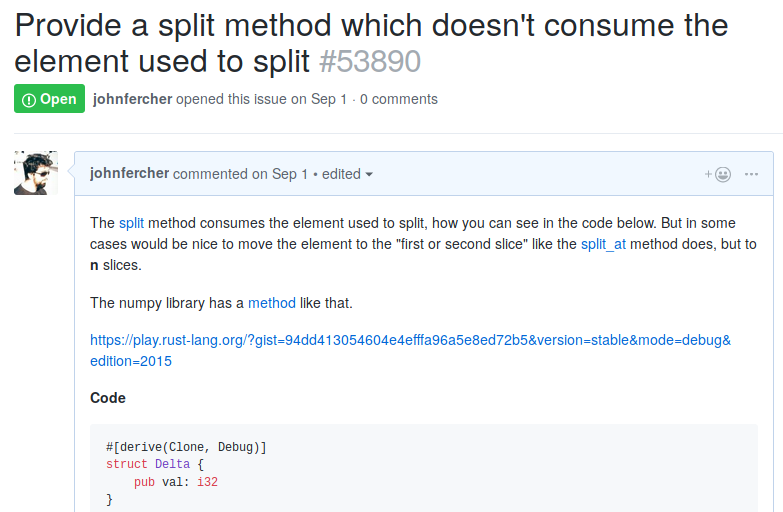
\includegraphics[width=10.0cm]{imgs/rfc.png}
	\end{center}
\end{frame}


\section{Quem usa em produção?}

\begin{frame}{Quem usa em produção?}
	\begin{itemize}
		\item Friends of Rust · The Rust Programming Language:
		\begin{itemize}
			\item https://www.rust-lang.org/pt-BR/friends.html
		\end{itemize}
	\end{itemize}
\end{frame}

\section{Programando em Rust}
\begin{frame}{Hello World}
	\begin{itemize}
		\item cargo new nome\_do\_projeto --bin
		\item cargo run
		\item cargo test
		\item cargo run --release
	\end{itemize}
	
	\vspace{1cm}
	
	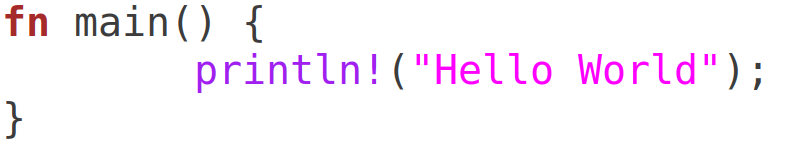
\includegraphics[width=6.0cm]{imgs/hello_world.png}	
\end{frame}

\begin{frame}{Mutabilidade x Imutabilidade}
	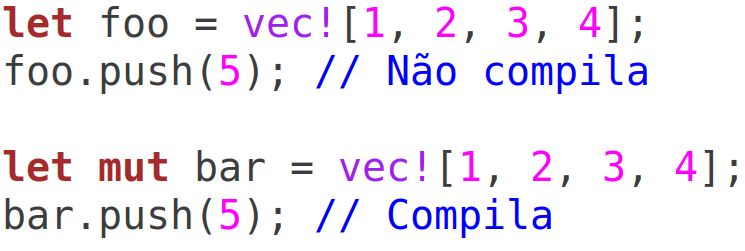
\includegraphics[width=5.5cm]{imgs/mut_x_imut.png}	
\end{frame}

%\begin{frame}{Ownership + Borrowing}
%	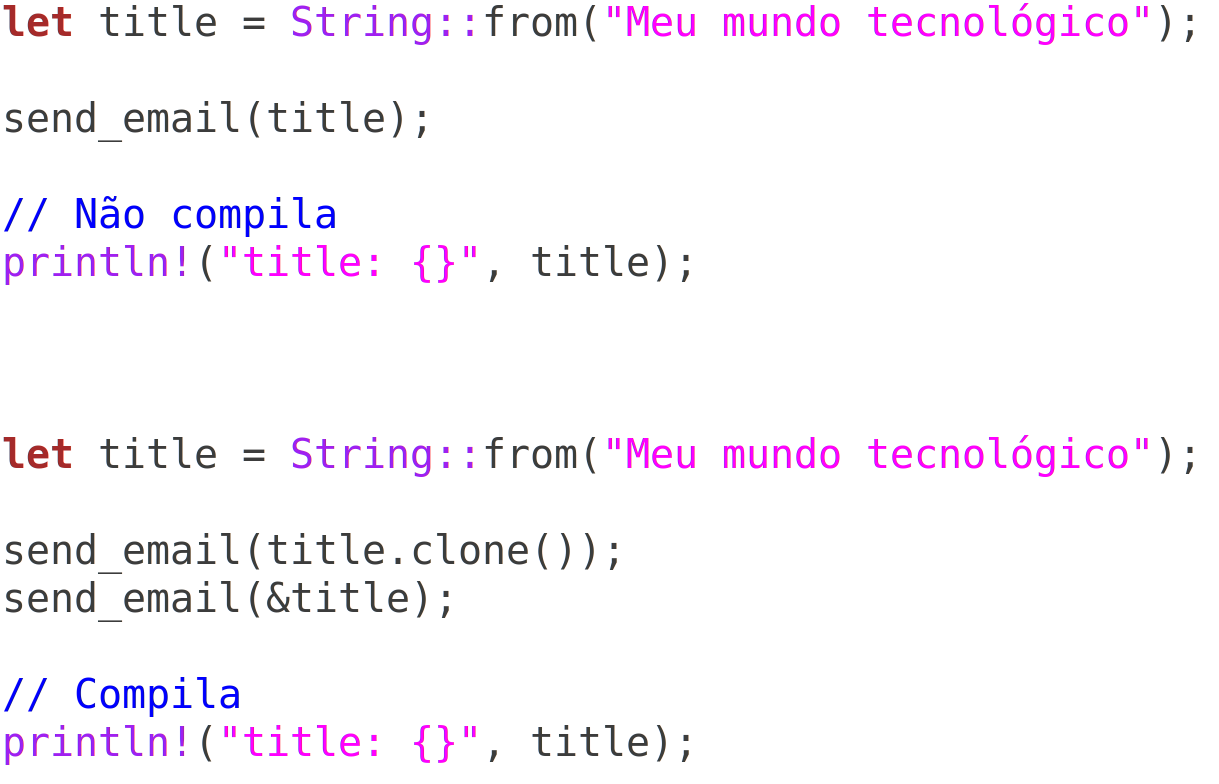
\includegraphics[width=9cm]{imgs/owership_borrowing.png}	
%\end{frame}

\begin{frame}{Thread-safe}
	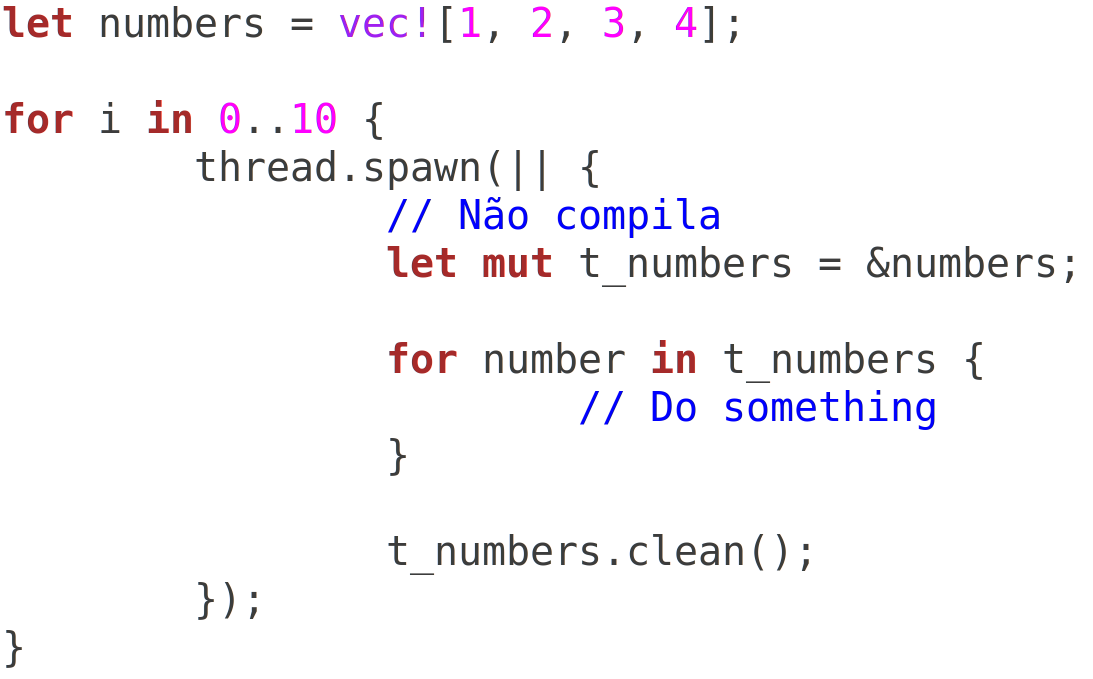
\includegraphics[width=8.5cm]{imgs/thread_safe.png}	
\end{frame}

\begin{frame}{3 Formas de Filtrar uma Lista}
	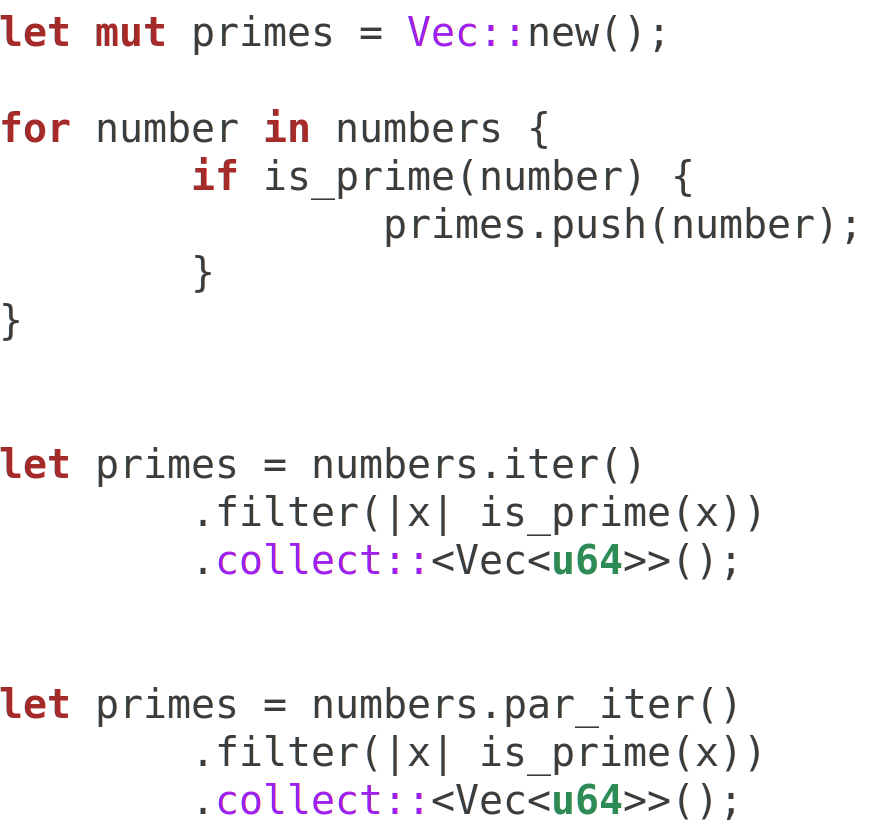
\includegraphics[width=6.8cm]{imgs/filter_list.png}	
\end{frame}

\begin{frame}{Benchmark Para 150.000 Números}
	\begin{figure}
		\begin{tikzpicture}
		\begin{axis}[
		mbarplot,
		ymin=0, ymax=7233.0,
		%xlabel={Foo},
		ylabel={\scriptsize Tempo de Execução},
		width=0.9\textwidth,
		height=8cm,
		xticklabels={,,}
		]
		
		\addplot+[gray] plot coordinates {(0, 7233.0)};
		\addplot+[black] plot coordinates {(0, 6916.0)};
		\addplot+[purple] plot coordinates {(0, 2073.0)};
		
		\legend{ForLoop (7233s), Iterator (6916s), ParallelIterator (2073s)}
		
		\end{axis}
		\end{tikzpicture}
	\end{figure}
\end{frame}

\begin{frame}{Limitando o Paralelismo}
	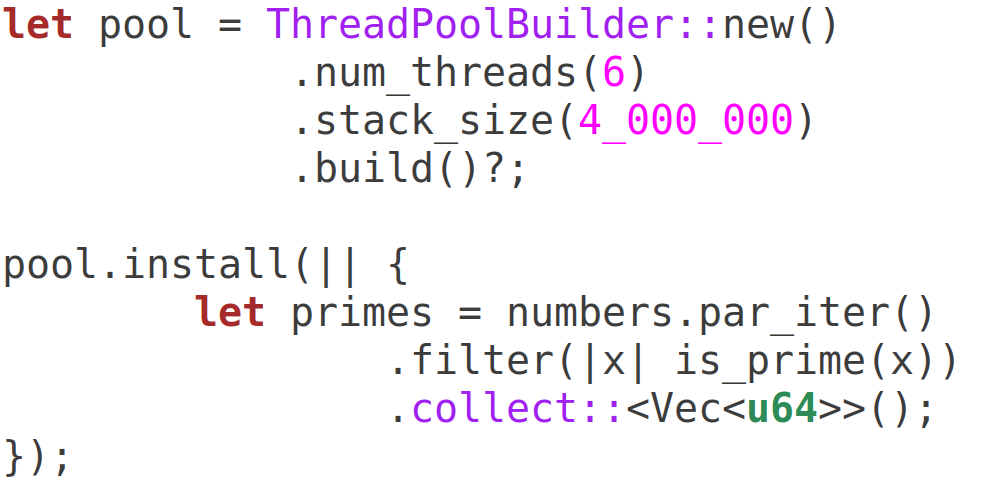
\includegraphics[width=7.5cm]{imgs/limit_threds.png}	
\end{frame}

\begin{frame}[noframenumbering]{Rust para paralelismo...}
	\begin{center}
		
\includegraphics[width=10.0cm]{imgs/choque_de_cultura_04.jpg}	
	\end{center}
\end{frame}


\begin{frame}{Gerenciador de pacotes}
	Cargo.TOML
	
	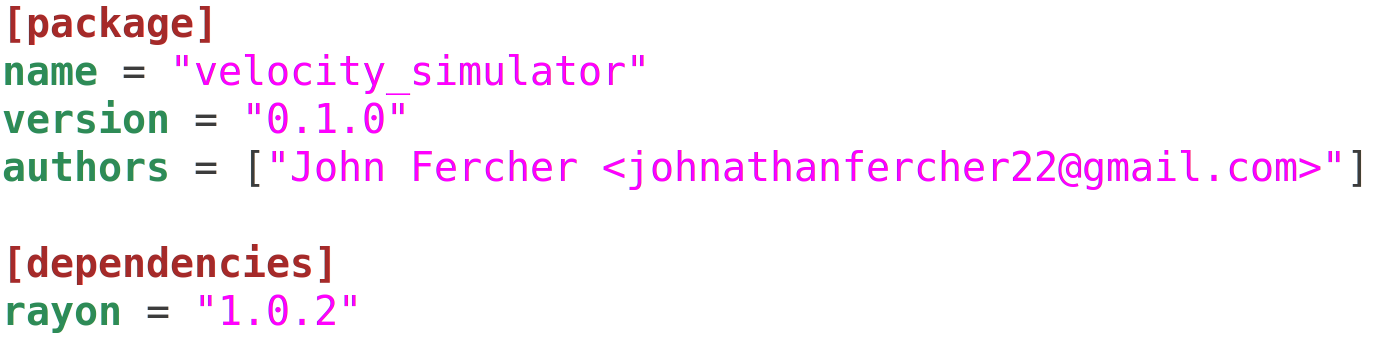
\includegraphics[width=10cm]{imgs/cargo.png}	
\end{frame}

\begin{frame}{Testes unitários}
	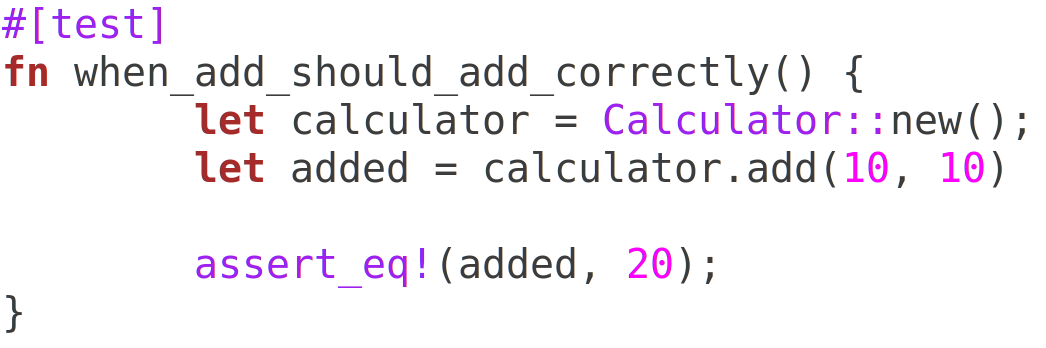
\includegraphics[width=8cm]{imgs/unit_tests.png}	
\end{frame}

\begin{frame}{IDEs: JetBrains, Visual Studio Code, ...}
	\begin{center}
		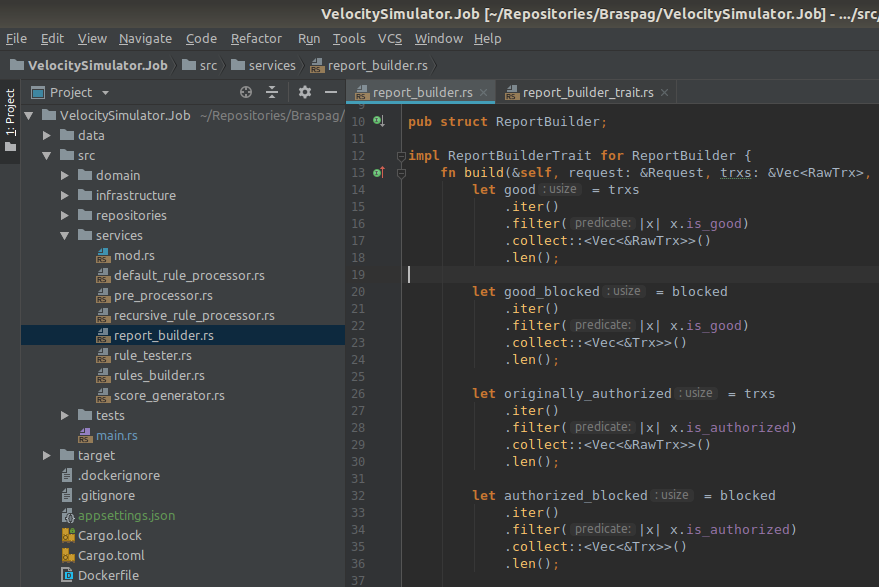
\includegraphics[width=11cm]{imgs/ide.png}	
	\end{center}
\end{frame}

\begin{frame}{Dockerfile}
	\begin{center}
		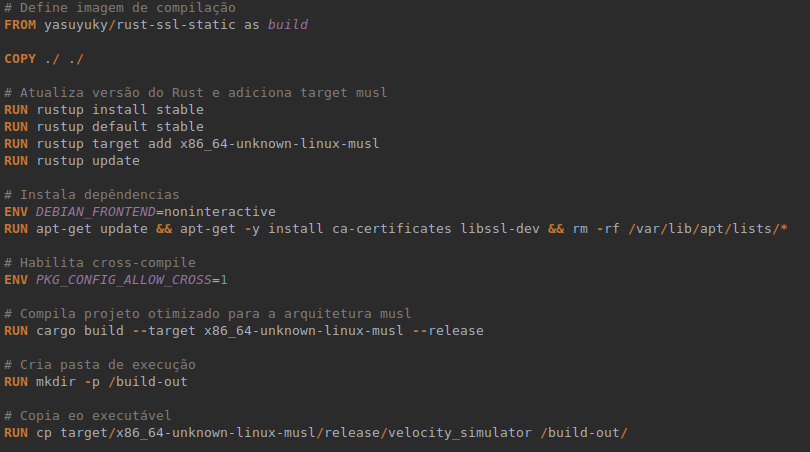
\includegraphics[width=11cm]{imgs/dockerfile1.png}	
	\end{center}
\end{frame}

\begin{frame}[noframenumbering]{Dockerfile}
	\begin{center}
		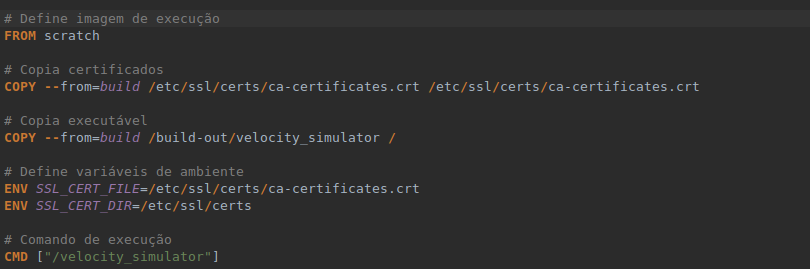
\includegraphics[width=11cm]{imgs/dockerfile2.png}	
	\end{center}
\end{frame}

\begin{frame}[noframenumbering]{Dockerfile}
	\begin{center}
		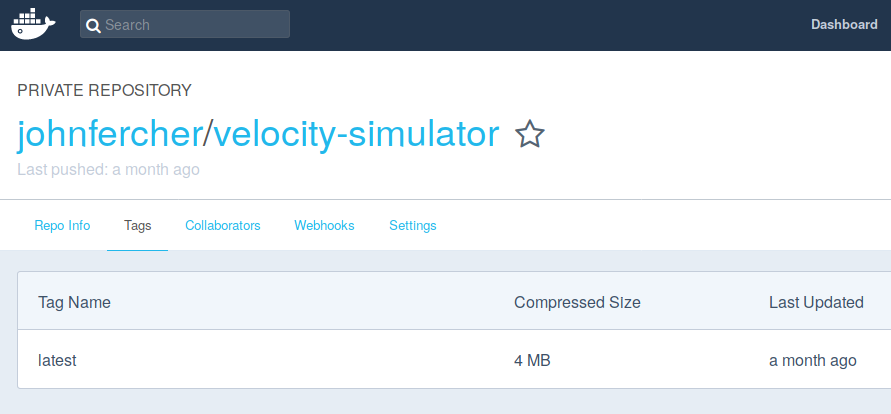
\includegraphics[width=12cm]{imgs/dockerfile3.png}	
	\end{center}
\end{frame}

\section{Resolução de um problema}

\begin{frame}{Velocity}
	Regras de repetição:
	\begin{itemize}
		\item 5 repetições de um \textbf{Cpf} em 10 minutos;
		\item 10 repetições de um \textbf{Cartão} em 2 dias;
		\item 2 repetições de um \textbf{Ip} em 5 minutos;
	\end{itemize}
	
	\begin{chronology}[5]{1}{10}{80ex}[\textwidth]
		\event{1}{\textbf{1 min:} 127.0.0.1}
		\event{4}{\textbf{4 min:} 127.0.0.1}
		\event{7}{\textbf{7 min:} 127.0.0.1}
		\event{8}{\textcolor{red}{\textbf{8 min:} 127.0.0.1}}
	\end{chronology}
\end{frame}

\begin{frame}{Provas de Conceito}
	\begin{center}
		
\includegraphics[width=9.0cm]{imgs/battle.png}	
	\end{center}
\end{frame}

\begin{frame}{Sobre os Benchmarks V1.0}	
	\textbf{Hardware: I7 8770 (6 núcleos + 6 threads), 8GB RAM DDR4, SSD;}
	
	\begin{itemize}
		\item Não é utilizado nenhuma técnica de agrupamento;
		\item Não é utilizado nenhum artifício de programação funcional;
	\end{itemize}
\end{frame}

\begin{frame}{Benchmark (v1.0)}
	\begin{figure}
		\begin{tikzpicture}
		\begin{axis}[
		mbarplot,
		ymin=0, ymax=1280.0,
		%xlabel={Foo},
		ylabel={\scriptsize Tempo de Execução},
		width=0.9\textwidth,
		height=8cm,
		xticklabels={,,}
		]
		
		\addplot+[gray] plot coordinates {(0, 1280.0)};
		
		\legend{R (1280m)}
		
		\end{axis}
		\end{tikzpicture}
	\end{figure}
\end{frame}

\begin{frame}[noframenumbering]{Benchmark (v1.0)}
	\begin{figure}
		\begin{tikzpicture}
		\begin{axis}[
		mbarplot,
		ymin=0, ymax=1280.0,
		%xlabel={Foo},
		ylabel={\scriptsize Tempo de Execução},
		width=0.9\textwidth,
		height=8cm,
		xticklabels={,,}
		]
		
		\addplot+[gray] plot coordinates {(0, 1280.0)};
		\addplot+[black] plot coordinates {(0, 300.0)};
		
		\legend{R (1280m), C\# (300m)}
		
		\end{axis}
		\end{tikzpicture}
	\end{figure}
\end{frame}

\begin{frame}[noframenumbering]{Benchmark (v1.0)}
	\begin{figure}
		\begin{tikzpicture}
		\begin{axis}[
		mbarplot,
		ymin=0, ymax=1280.0,
		%xlabel={Foo},
		ylabel={\scriptsize Tempo de Execução},
		width=0.9\textwidth,
		height=8cm,
		xticklabels={,,}
		]
		
		\addplot+[gray] plot coordinates {(0, 1280.0)};
		\addplot+[black] plot coordinates {(0, 300.0)};
		\addplot+[purple] plot coordinates {(0, 10.0)};
		
		\legend{R (1280m), C\# (300m), Rust (10m)}
		
		\end{axis}
		\end{tikzpicture}
	\end{figure}
\end{frame}

\begin{frame}[noframenumbering]{Benchmark (v1.0)}
	\begin{center}
		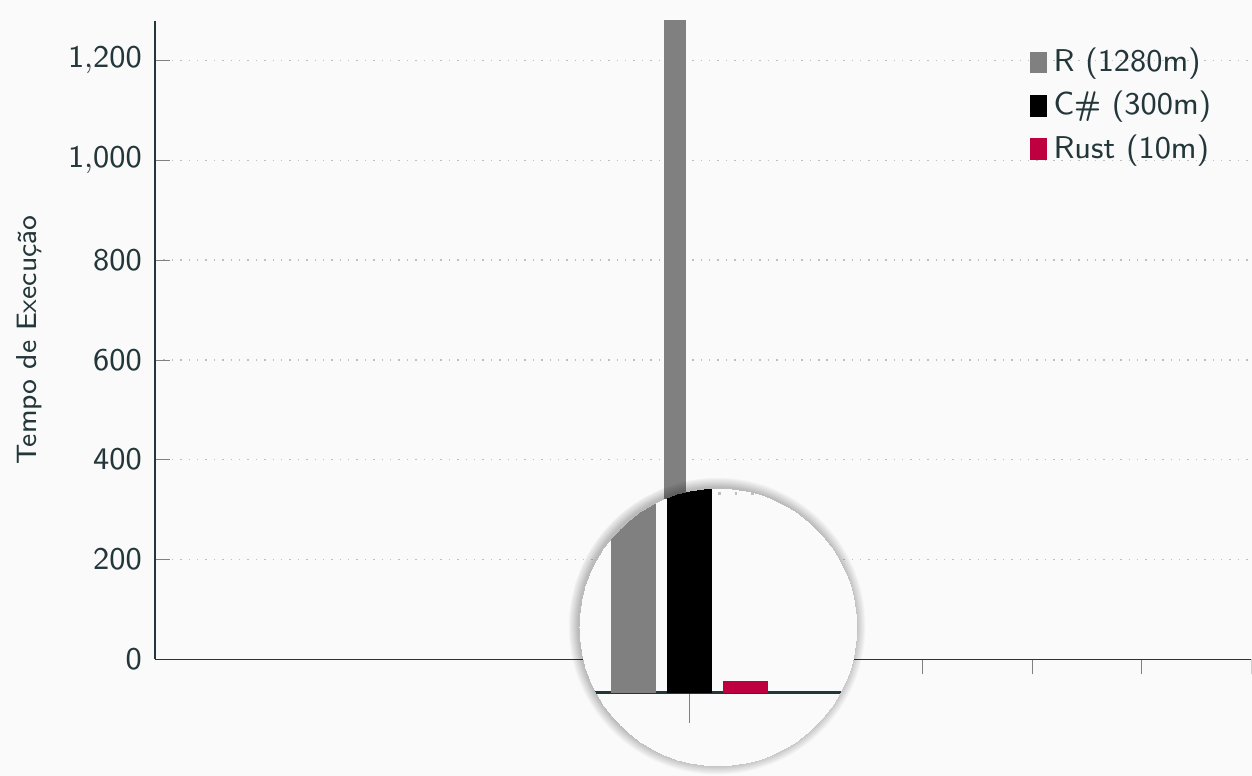
\includegraphics[width=12.8cm]{imgs/bench1zoom.png}	
	\end{center}
\end{frame}

\begin{frame}[noframenumbering]{Benchmark (v1.0)}
	\begin{center}
		
\includegraphics[width=10.0cm]{imgs/choque_de_cultura_01.jpg}	
	\end{center}
\end{frame}

\begin{frame}{Sobre os Benchmarks V2.0}	
	\textbf{Hardware: I7 8770 (6 núcleos + 6 threads), 8GB RAM DDR4, SSD;}
	
	\begin{itemize}
		\item Todos os algoritmos utilizam agrupamento;
		\item Rust e Python utilizam programação funcional;
		\item Python utiliza a lib Numpy, que é feita em C, C++ e Fortran;
	\end{itemize}
\end{frame}

\begin{frame}{Benchmark (v2.0)}
	\begin{figure}
		\begin{tikzpicture}
		\begin{axis}[
		mbarplot,
		ymin=0, ymax=1800.0,
		%xlabel={Foo},
		ylabel={\scriptsize Tempo de Execução},
		width=0.9\textwidth,
		height=8cm,
		xticklabels={,,}
		]
		
		\addplot+[gray] plot coordinates {(0, 1800.0)};
		
		\legend{SQL (1800s)}
		
		\end{axis}
		\end{tikzpicture}
	\end{figure}
\end{frame}

\begin{frame}[noframenumbering]{Benchmark (v2.0)}
	\begin{figure}
		\begin{tikzpicture}
		\begin{axis}[
		mbarplot,
		ymin=0, ymax=1800.0,
		%xlabel={Foo},
		ylabel={\scriptsize Tempo de Execução},
		width=0.9\textwidth,
		height=8cm,
		xticklabels={,,}
		]
		
		\addplot+[gray] plot coordinates {(0, 1800.0)};
		\addplot+[orange] plot coordinates {(0, 88.0)};
		
		\legend{SQL (1800s), Python (88s)}
		
		\end{axis}
		\end{tikzpicture}
	\end{figure}
\end{frame}

\begin{frame}[noframenumbering]{Benchmark (v2.0)}
	\begin{figure}
		\begin{tikzpicture}
		\begin{axis}[
		mbarplot,
		ymin=0, ymax=1800.0,
		%xlabel={Foo},
		ylabel={\scriptsize Tempo de Execução},
		width=0.9\textwidth,
		height=8cm,
		xticklabels={,,}
		]
		
		\addplot+[gray] plot coordinates {(0, 1800.0)};
		\addplot+[orange] plot coordinates {(0, 88.0)};
		\addplot+[purple] plot coordinates {(0, 5.0)};
		
		\legend{SQL (1800s), Python (88s), Rust (5s)}
		
		\end{axis}
		\end{tikzpicture}
	\end{figure}
\end{frame}

\begin{frame}[noframenumbering]{Benchmark (v2.0)}
	\begin{center}
		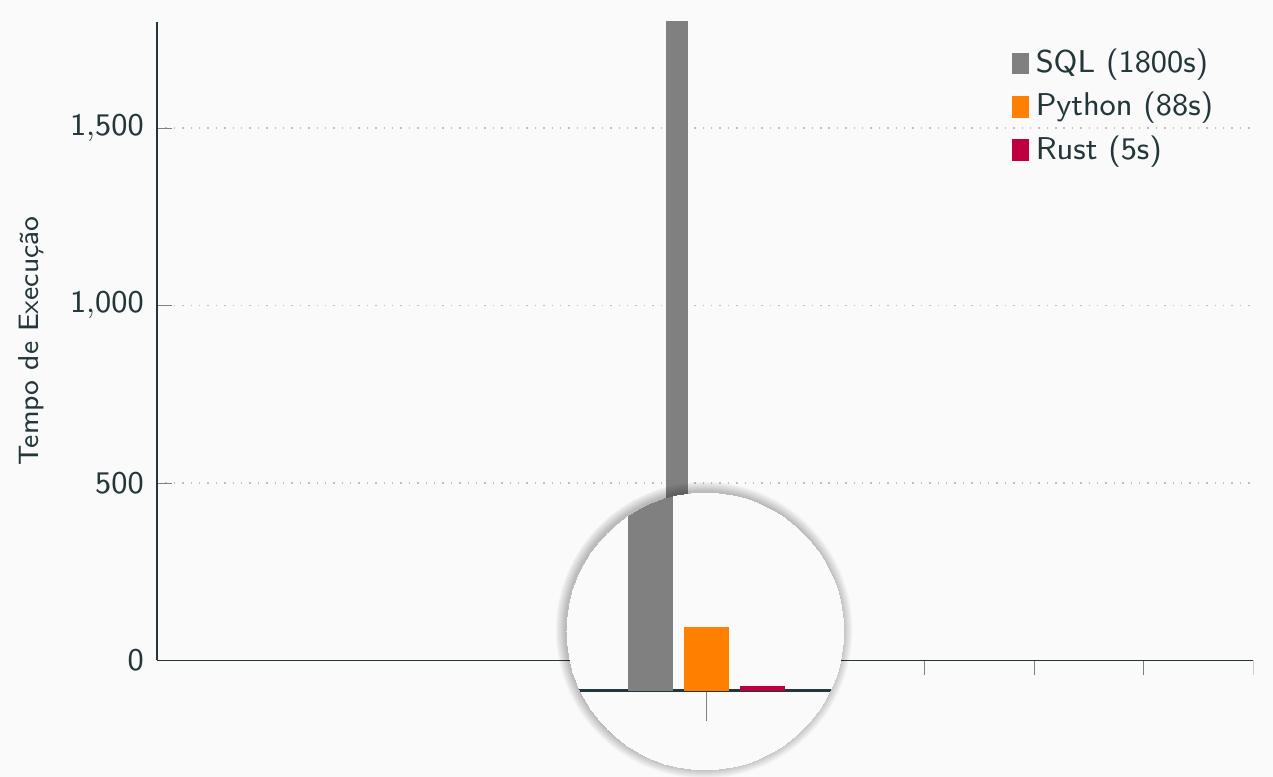
\includegraphics[width=12.8cm]{imgs/bench2zoom.png}	
	\end{center}
\end{frame}

\begin{frame}[noframenumbering]{Benchmark (v2.0)}
	\begin{center}
		
\includegraphics[width=10.0cm]{imgs/choque_de_cultura_02.jpg}	
	\end{center}
\end{frame}

\begin{frame}{Conclusões}	
	\begin{itemize}
		\item Rust é uma linguagem recente, porém, completa em relação as ferramentas de desenvolvimento;
		\item Indicada para resolver problemas de processamento pesado (competindo com C, C++ e Fortran);
		\item Ótima para lidar com problemas que requerem paralelismo;
		\item Curva de aprendizado é grande;
	\end{itemize}	
\end{frame}

\begin{frame}[standout]
	\begin{center}
		
\includegraphics[width=2.5cm]{imgs/rustacean.png}
	\end{center}
  	Obrigado		
\end{frame}

\end{document}
